\documentclass[review]{elsarticle}

\usepackage{lineno,hyperref}
\modulolinenumbers[5]

% Package to change into landscape
\usepackage{pdflscape}

% Package for table
\usepackage{booktabs}

% For some math expression
\usepackage{amsmath}
\usepackage{mathabx}

% Package for SI units
\usepackage{siunitx}

%% figure package
\usepackage{epsf,graphicx}
\usepackage{epstopdf}
\usepackage{subfigure} 

% Define the operator of convolution
\newcommand{\Conv}{\mathop{\scalebox{1.5}{\raisebox{-0.2ex}{$\ast$}}}}%

% Use the acro package to handle the acronym
\usepackage{acro}
%\acrodef{cap}[CaP]{prostate cancer}
\DeclareAcronym{cap}{
short = PCa,
long = Prostate Cancer
}
%\acrodef{cade}[CADe]{computer-aided detection}
\DeclareAcronym{cade}{
short = CADe,
long = Computer-Aided Detection
}
%\acrodef{cadx}[CADx]{computer-aided diagnosis}
\DeclareAcronym{cadx}{
short = CADx,
long = Computer-Aided Diagnosis
}
%\acrodef{us}[US]{ultrasound}
\DeclareAcronym{us}{
short = US,
long = UltraSound
}
%\acrodef{ct}[CT]{computer tomography}
\DeclareAcronym{ct}{
short = CT,
long = Computer Tomography
}
%\acrodef{cad}[CAD]{computer-aided detection and diagnosis}
\DeclareAcronym{cad}{
short = CAD,
long = Computer-Aided Detection and Diangosis
}
%\acrodef{mri}[MRI]{magnetic resonance imaging}
\DeclareAcronym{mri}{
short = MRI,
long = Magnetic Resonance Imaging
}
%\acrodef{nmr}[NMR]{nuclear magnetic resonance}
\DeclareAcronym{nmr}{
short = NMR,
long = Nuclear Magnetic Resonance
}
%\acrodef{t2w}[T$_2$-W]{T$_2$ Weighted}
\DeclareAcronym{t2w}{
short = T$_2$-W,
long = T$_2$ Weighted
}
%\acrodef{dce}[DCE]{dynamic contrast-enhanced}
\DeclareAcronym{dce}{
short = DCE,
long = Dynamic Contrast-Enhanced
}
%\acrodef{dw}[DW]{diffusion weighted}
\DeclareAcronym{dw}{
short = DW,
long = Diffusion Weighted
}
%\acrodef{mrsi}[MRSI]{magnetic resonance spectroscopy imaging}
\DeclareAcronym{mrsi}{
short = MRSI,
long = Magnetic Resonance Spectroscopy Imaging
}
%\acrodef{bph}[BPH]{benign prostatic hyperplasia}
\DeclareAcronym{bph}{
short = BPH,
long = Benign Prostatic Hyperplasia
}
%\acrodef{pz}[PZ]{peripheral zone}
\DeclareAcronym{pz}{
short = PZ,
long = Peripheral Zone
}
%\acrodef{cz}[CZ]{central zone}
\DeclareAcronym{cz}{
short = CZ,
long = Central Zone
}
%\acrodef{tz}[TZ]{transitional zone}
\DeclareAcronym{tz}{
short = TZ,
long = Transitional Zone
}
%\acrodef{cg}[CG]{central gland}
\DeclareAcronym{cg}{
short = CG,
long = Central Gland
}
%\acrodef{psa}[PSA]{prostate-specific antigen}
\DeclareAcronym{psa}{
short = PSA,
long = Prostate-Specific Antigen
}
%\acrodef{trus}[TRUS]{transrectal ultrasound}
\DeclareAcronym{trus}{
short = TRUS,
long = Transrectal UltraSound
}
%\acrodef{tr}[TR]{repetition time}
\DeclareAcronym{tr}{
short = TR,
long = Repetition Time
}
%\acrodef{te}[TE]{echo time}
\DeclareAcronym{te}{
short = TE,
long = Echo Time
}
%\acrodef{si}[SI]{signal intensity}
\DeclareAcronym{si}{
short = SI,
long = Signal Intensity
}
%\acrodef{ees}[EES]{extravascular-extracellular space}
\DeclareAcronym{ees}{
short = EES,
long = Extravascular-Extracellular Space
}
%\acrodef{t1w}[T$_1$-W]{T$_1$ Weighted}
\DeclareAcronym{t1w}{
short = T$_1$-W,
long = T$_1$ Weighted
}
%\acrodef{fse}[FSE]{Fast Spin-Echo}
\DeclareAcronym{fse}{
short = FSE,
long = Fast Spin-Echo
}
%\acrodef{adc}[ADC]{Apparent Diffusion Coeffient}
\DeclareAcronym{adc}{
short = ADC,
long = Apparent Diffusion Coefficient
}
%\acrodef{roi}[ROI]{region of interest}
\DeclareAcronym{roi}{
short = ROI,
long = Region Of Interest
}
%\acrodef{cse}[CSE]{chemical shift effect}
\DeclareAcronym{cse}{
short = CSE,
long = Chemical Shift Effect
}
%\acrodef{snr}[SNR]{signal-to-noise}
\DeclareAcronym{snr}{
short = SNR,
long = Signal-to-Noise
}
%\acrodef{gs}[GS]{Gleason score}
\DeclareAcronym{gs}{
short = GS,
long = Gleason Score
}
%\acrodef{ersspc}[ERSSPC]{European Randomized Study of Screening for Prostate Cancer}
\DeclareAcronym{ersspc}{
short = ERSSPC,
long = European Randomized Study of Screening for Prostate Cancer
}
%\acrodef{plco}[PLCO]{Prostate, Lung, Colorectal and Ovarian}
\DeclareAcronym{plco}{
short = PLCO,
long = Prostate Lung Colorectal and Ovarian
}
%\acrodef{fig}[Fig.]{figure}
\DeclareAcronym{fig}{
short = Fig.,
long = figure
}
\DeclareAcronym{tab}{
short = Table,
long = table
}
\DeclareAcronym{eq}{
short = Eq.,
long = equation
}
\DeclareAcronym{sec}{
short = Sect.,
long = section
}
\DeclareAcronym{fov}{
short = FOV,
long = Field Of View
}
\DeclareAcronym{dwt}{
short = DWT,
long = Discrete Wavelet Transform
}
\DeclareAcronym{dwst}{
short = DWST,
long = Discrete Wavelet Squared Transform
}
\DeclareAcronym{map}{
short = MAP,
long = Maximum \textit{a posteriori}
}
\DeclareAcronym{ml}{
short = ML,
long = Maximum Likelihood
}
\DeclareAcronym{mrf}{
short = MRF,
long = Markov Random Field
}
\DeclareAcronym{itk}{
short = ITK,
long = Insight Segmentation and Registration Toolkit
}
\DeclareAcronym{es}{
short = ES,
long = Evolution Strategy
}
\DeclareAcronym{pdf}{
short = PDF,
long = Probability Density Function
}
\DeclareAcronym{gscale}{
short = \textit{g}-scale,
long = generalized scale
}
\DeclareAcronym{aif}{
short = AIF,
long = Arterial Input Function
}
\DeclareAcronym{svd}{
short = SVD,
long = Singular Value Decomposition
}
\DeclareAcronym{mse}{
short = MSE,
long = Mean Squared Error
}
\DeclareAcronym{mi}{
short = MI,
long = Mutual Information
}
\DeclareAcronym{mantra}{
short = MANTRA,
long = Multi-Attribute Non-initializing Texture Reconstruction based Active shape model
}
\DeclareAcronym{asm}{
short = ASM,
long = Active Shape Model
}
\DeclareAcronym{pca}{
short = PCA,
long = Principal Components Aanalysis
}
\DeclareAcronym{weritas}{
short = WERITAS,
long = Weighted Ensemble of Regional Image Textures for Active shape model Segmentation
}
\DeclareAcronym{staple}{
short = STAPLE,
long = Simultaneous Truth and Performance Level Estimation
}
\DeclareAcronym{lda}{
short = LDA,
long = Linear Discriminant Analysis
}
\DeclareAcronym{lbp}{
short = LBP,
long = Local Binary Pattern
}
\DeclareAcronym{tps}{
short = TPS,
long = Thin Plate Spline
}
\DeclareAcronym{acm}{
short = ACM,
long = Active Contour Model
}
\DeclareAcronym{cmi}{
short = CMI,
long = Combined Mutual Information
}
\DeclareAcronym{svm}{
short = SVM,
long = Support Vector Machines
}
\DeclareAcronym{rvm}{
short = RVM,
long = Relevant Vector Machine
}
\DeclareAcronym{rbf}{
short = RBF,
long = Radial Basis Function
}
\DeclareAcronym{knn}{
short = $k$-NN,
long = $k$-Neareast Neighbour
}
\DeclareAcronym{dct}{
short = DCT,
long = Discrete Cosine Transform
}
\DeclareAcronym{hog}{
short = HOG,
long = Histogram of Oriented Gradient
}
\DeclareAcronym{dft}{
short = DFT,
long = Discrete Fourier Transform
}
\DeclareAcronym{mrmr}{
short = mRMR,
long = minimum Redundancy Maximum Relevance
}
\DeclareAcronym{lle}{
short = LLE,
long = Locally Linear Embedding
}
\DeclareAcronym{ica}{
short = ICA,
long = Independent Components Analysis
}
\DeclareAcronym{qda}{
short = QDA,
long = Quadratic Discriminant Analysis
}
\DeclareAcronym{id3}{
short = ID3,
long = Iterative Dichotomiser 3
}
\DeclareAcronym{cart}{
short = CART,
long = Classification and Regression Tree
}
\DeclareAcronym{bagging}{
short = bagging,
long = bootsrap aggregating
}
\DeclareAcronym{loo}{
short = LOOCV,
long = Leave-One-Out Cross-Validation
}
\DeclareAcronym{kcv}{
short = $k$-CV,
long = $k$-fold Cross-Validation
}
\DeclareAcronym{roc}{
short = ROC,
long = Receiver Operating Characteristic
}
\DeclareAcronym{froc}{
short = FROC,
long = Free-Response Receiver Operating Characteristic
}
\DeclareAcronym{auc}{
short = AUC,
long = Area Under the Curve
}
\DeclareAcronym{pun}{
short = PUN,
long = Phenomenological Universalities
}
\DeclareAcronym{mpmri}{
short = mpMRI,
long = multiparametric \ac{mri}
}
\DeclareAcronym{pd}{
short = PD,
long = Proton Density
}
\DeclareAcronym{nb}{
short = NB,
long = Naive Bayes
}
\DeclareAcronym{rf}{
short = RF,
long = Random Forest
}

%%% Local Variables: 
%%% mode: latex
%%% TeX-master: "../main"
%%% End: 


\journal{Medical Image Analysis}

%%%%%%%%%%%%%%%%%%%%%%%
%% Elsevier bibliography styles
%%%%%%%%%%%%%%%%%%%%%%%
%% To change the style, put a % in front of the second line of the current style and
%% remove the % from the second line of the style you would like to use.
%%%%%%%%%%%%%%%%%%%%%%%

%% Numbered
%\bibliographystyle{00_files_system/model1-num-names}

%% Numbered without titles
%\bibliographystyle{00_files_system/model1a-num-names}

%% Harvard
\bibliographystyle{00_files_system/model2-names}\biboptions{authoryear}

%% Vancouver numbered
%\usepackage{00_files_system/numcompress}\bibliographystyle{00_files_system/model3-num-names}

%% Vancouver name/year
%\usepackage{numcompress}\bibliographystyle{00_files_system/model4-names}\biboptions{authoryear}

%% APA style
%\bibliographystyle{00_files_system/model5-names}\biboptions{authoryear}

%% AMA style
%\usepackage{numcompress}\bibliographystyle{00_files_system/model6-num-names}

%% `Elsevier LaTeX' style
%\bibliographystyle{elsarticle-num}
%%%%%%%%%%%%%%%%%%%%%%%

\begin{document}

\begin{frontmatter}

\title{Automatic prostate cancer detection through \acs*{dce}-\acs*{mri} images: all you need is a good normalization}

% Add authors and the different addresses
\author[label1,label3]{Guillaume~Lema\^itre\corref{cor1}}
\ead{g.lemaitre58@gmail.com}
\author[label3]{Robert~Mart\'i}
%\ead{marly@eia.udg.edu}
%\author[label3]{Jordi~Freixenet}
%\ead{jordif@eia.udg.edu}
%\author[label5]{Anke Meyer-Baese}
%\ead{ameyerbaese@fsu.edu}
%\author[label4]{Joan~C.~Vilanova}
%\ead{kvilanova@comg.cat}
%\author[label2]{Paul~M.~Walker}
%\ead{pwalker@u-bourgogne.fr}
\author[label1,label6]{Fabrice~Meriaudeau}
%\ead{fabrice.meriaudeau@u-bourgogne.fr}
\address[label1]{\scriptsize LE2I UMR6306, CNRS, Arts et M\'etiers, Univ. Bourgogne Franche-Comt\'e, 12 rue de la Fonderie, 71200 Le Creusot, France}
%\address[label2]{\scriptsize LE2I UMR6306, CNRS, Arts et M\'etiers, Univ. Bourgogne Franche-Comt\'e, Avenue Alain Savary, 21000 Dijon, France}
\address[label3]{\scriptsize ViCOROB, Universitat de Girona, Campus Montilivi, Edifici P4, 17071 Girona, Spain}
%\address[label4]{\scriptsize Department of Magnetic Resonance, Cl\'inica Girona, Lorenzana 36, 17002 Girona, Spain}
%\address[label5]{\scriptsize Department of Scientific Computing, 400 Dirac Science Library, Florida State University, Tallahassee, FL 32306, United States}
\address[label6]{\scriptsize CISIR, Electrical \& Electronic Engineering Department, Universiti Teknologi Petronas, 32610 Seri Iskandar, Perak, Malaysia}
\cortext[cor1]{Corresponding author.}

% Start the abstract
\begin{abstract}
This template helps you to create a properly formatted \LaTeX\ manuscript.
\end{abstract}

% Give the different keywords
\begin{keyword}
\acs*{dce}-\acs*{mri}\sep prostate cancer\sep normalization\sep classification\sep quantification
\end{keyword}

\end{frontmatter}

% Reset all the acronyms
\acresetall
\linenumbers
% Include now the different files
\section{Introduction}

\Ac{cap} is the second most frequently diagnosed men cancer, accounting for 899,000 cases leading to 258,100 deaths~\citep{ferlay2010estimates}.
As highlighted by the PI-RADS Steering Committee, the two main challenges to be addressed are~\citep{weinreb2016pi}:
(i) the improvement of detecting clinically significant \ac{cap} and
(ii) an increase of the confidence in benign or dormant cases, avoiding unnecessary invasive medical exams.
In this regard, \ac{mpmri} is frequently used to build robust \ac{cad} systems to detect, localize, and grade \ac{cap}.
In general, \ac{cad} systems are based on \ac{mpmri} which potentially combines several of the following modalities~\citep{lemaitre2015computer}: \ac{t2w}-\ac{mri}, \ac{dce}-\ac{mri}, \ac{adc} maps, and \ac{mrsi}.

In \ac{dce}-\ac{mri}, a contrast media is injected intravenously and a set of images is acquired over time.
Consequently, each voxel in an image corresponds to a dynamic signal which is related to both contrast agent concentration and the vascular properties of the tissue.
Therefore, changes of the enhanced signal allows to discriminate healthy from \ac{cap} tissues.
In fact, these properties are automatically extracted using quantitative or semi-quantitative approaches~\citep{lemaitre2015computer}.

\emph{Quantitative} approaches uses pharmacokinetic modelling based on a bicompartment model, namely Brix~\citep{brix1991pharmacokinetic} and Tofts~\citep{tofts1995quantitative} models.
The parameters of the Brix model are inferred assuming a linear relationship between the media concentration and the \ac{mri} signal intensity.
This assumption has shown, however, to lead to inaccurately estimate the pharmacokinetic parameters~\citep{heilmann2006determination}.
In the contrary, Tofts model requires a conversion from \ac{mri} signal intensity to concentration, which becomes a non-linear relationship using specific equation of \ac{mri} sequences (e.g., FLASH sequence).
Tofts modelling suffers, however, from a higher complexity~\citep{gliozzi2011phenomenological}.
Indeed, the conversion using the non-linear approach requires to acquire a T$_1$ map which is not always possible during clinical examination.
Additionally, the parameter calculation requires the \ac{aif} which is challenging to measure and can also lead to an inaccurate estimation.

\emph{Semi-quantitative} approaches are rather mathematical than pharmacokinetic modelling since no pharmacokinetic assumption regarding the relation between the \ac{mri} signal and the contrast agent are made~\citep{huisman2001accurate,gliozzi2011phenomenological}.
These methods offer the advantages to not require any knowledge about the \ac{mri} sequence nor any conversion from signal intensity to concentration.
However, they present some limitations: the heuristic approach proposed by \citeauthor{huisman2001accurate} requires an initial estimate of the noise standard deviation of the signal as well as some manual tuning.

Nevertheless, all presented methods suffer from two major drawbacks:
(i) inter-patient variability and (ii) loss of information.
The inter-patient variability is mainly due to the acquisition process and consequently leads to generalization issue while applying a machine learning algorithm.
All previous methods extract few discriminative parameters to describe the \ac{dce}-\ac{mri} signal which might lead to a loss of information.
%(i) the inter-patient variability of the data lead to a variation of the parameters estimated and subsequently to poor classification performance while designing \ac{cad} systems, and
%(ii) only few parameters are used to characterize the dynamic signal implying that some information are discarded.

In this work, we propose a fully automatic normalization method for \ac{dce}-\ac{mri} that reduces the inter-patient variability of the data.
The benefit and simplicity of our approach will be shown by classifying the whole normalized \ac{dce}-\ac{mri} signal and comparing with the state-of-the-art quantitative and semi-quantitative methods.
Additionally, we will show that using this normalization approach in conjunction with the quantitative methods improves the classification performance of most of the models.
We also propose a new clustering-based method to segment enhanced signals from the arteries, later used to estimate an \ac{aif} as well as an alternative approach to estimate the parameters of the semi-quantitative model proposed by~\cite{huisman2001accurate}.

% The benefit of our approach will be shown while using quantitative and semi-quantitative approaches.
% Additionally, we show that using the whole normalized \ac{dce}-\ac{mri} signal is preferable to quantitative and semi-quantitative methods, leading to the best classification performance.

The paper is organized as follows:
Section~\ref{sec:norm} details our normalization strategy for \ac{dce}-\ac{mri} data.
Quantitative and semi-quantitative methods are summarized in Sect.\,\ref{sec:stateart} with insights about their implementations.
Section~\ref{sec:materials} gives information about the dataset used and provided source code.
Experiments and results to answer the previous stated challenges are reported in Sect.\,\ref{sec:experiments} while discussed in Sect.\,\ref{sec:discussions}, followed by a concluding section.
%Section~\ref{sec:methods} outlines our normalization strategy (Section~\ref{sec:norm}) as well as specificity regarding the state-of-the-art methods used for comparison (Section~\ref{sec:stateart}).
%The dataset, experiments, and results are reported in Section~\ref{sec:experiments} while discussed in Section~\ref{sec:discussions} followed by a concluding section.

%%% Local Variables: 
%%% mode: latex
%%% TeX-master: "../main"
%%% End: 

\section{Methods}\label{sec:method}

\subsection{Normalization of \ac{dce}-\ac{mri} images}\label{sec:norm}

\begin{figure}
  \centering
  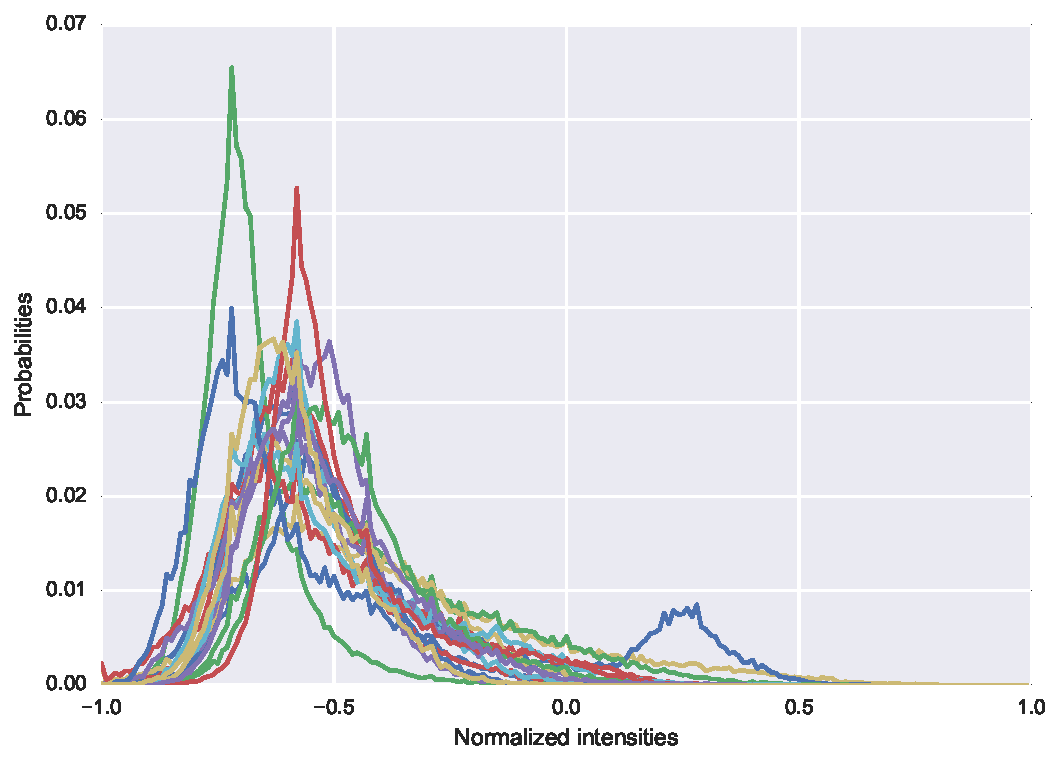
\includegraphics[width=0.7\linewidth]{02_methods/figures/t2w.pdf}
  \caption{Illustration of the inter-patient variations in 17 different patients, using the \acs*{pdf} representation.}
  \label{fig:t2w}
\end{figure}

In this work, we propose a method to normalize \ac{dce}-\ac{mri} prostate data to reduce inter-patient variations, although it can be applied to any \ac{dce}-\ac{mri} sequences.
In \ac{t2w}-\ac{mri}, these variations are characterized by a shift and a scaling of the intensities as illustrated by the intensity \ac{pdf} in Fig.\,\ref{fig:t2w}.
Therefore, these variations can be corrected using a $z$-score approach, assuming that the data follow a specific distribution~\citep{lemaitre2016normalization}.

\begin{figure*}
  \centering
  \hspace*{\fill}
  \subfigure[]{\label{subfig:pathhist}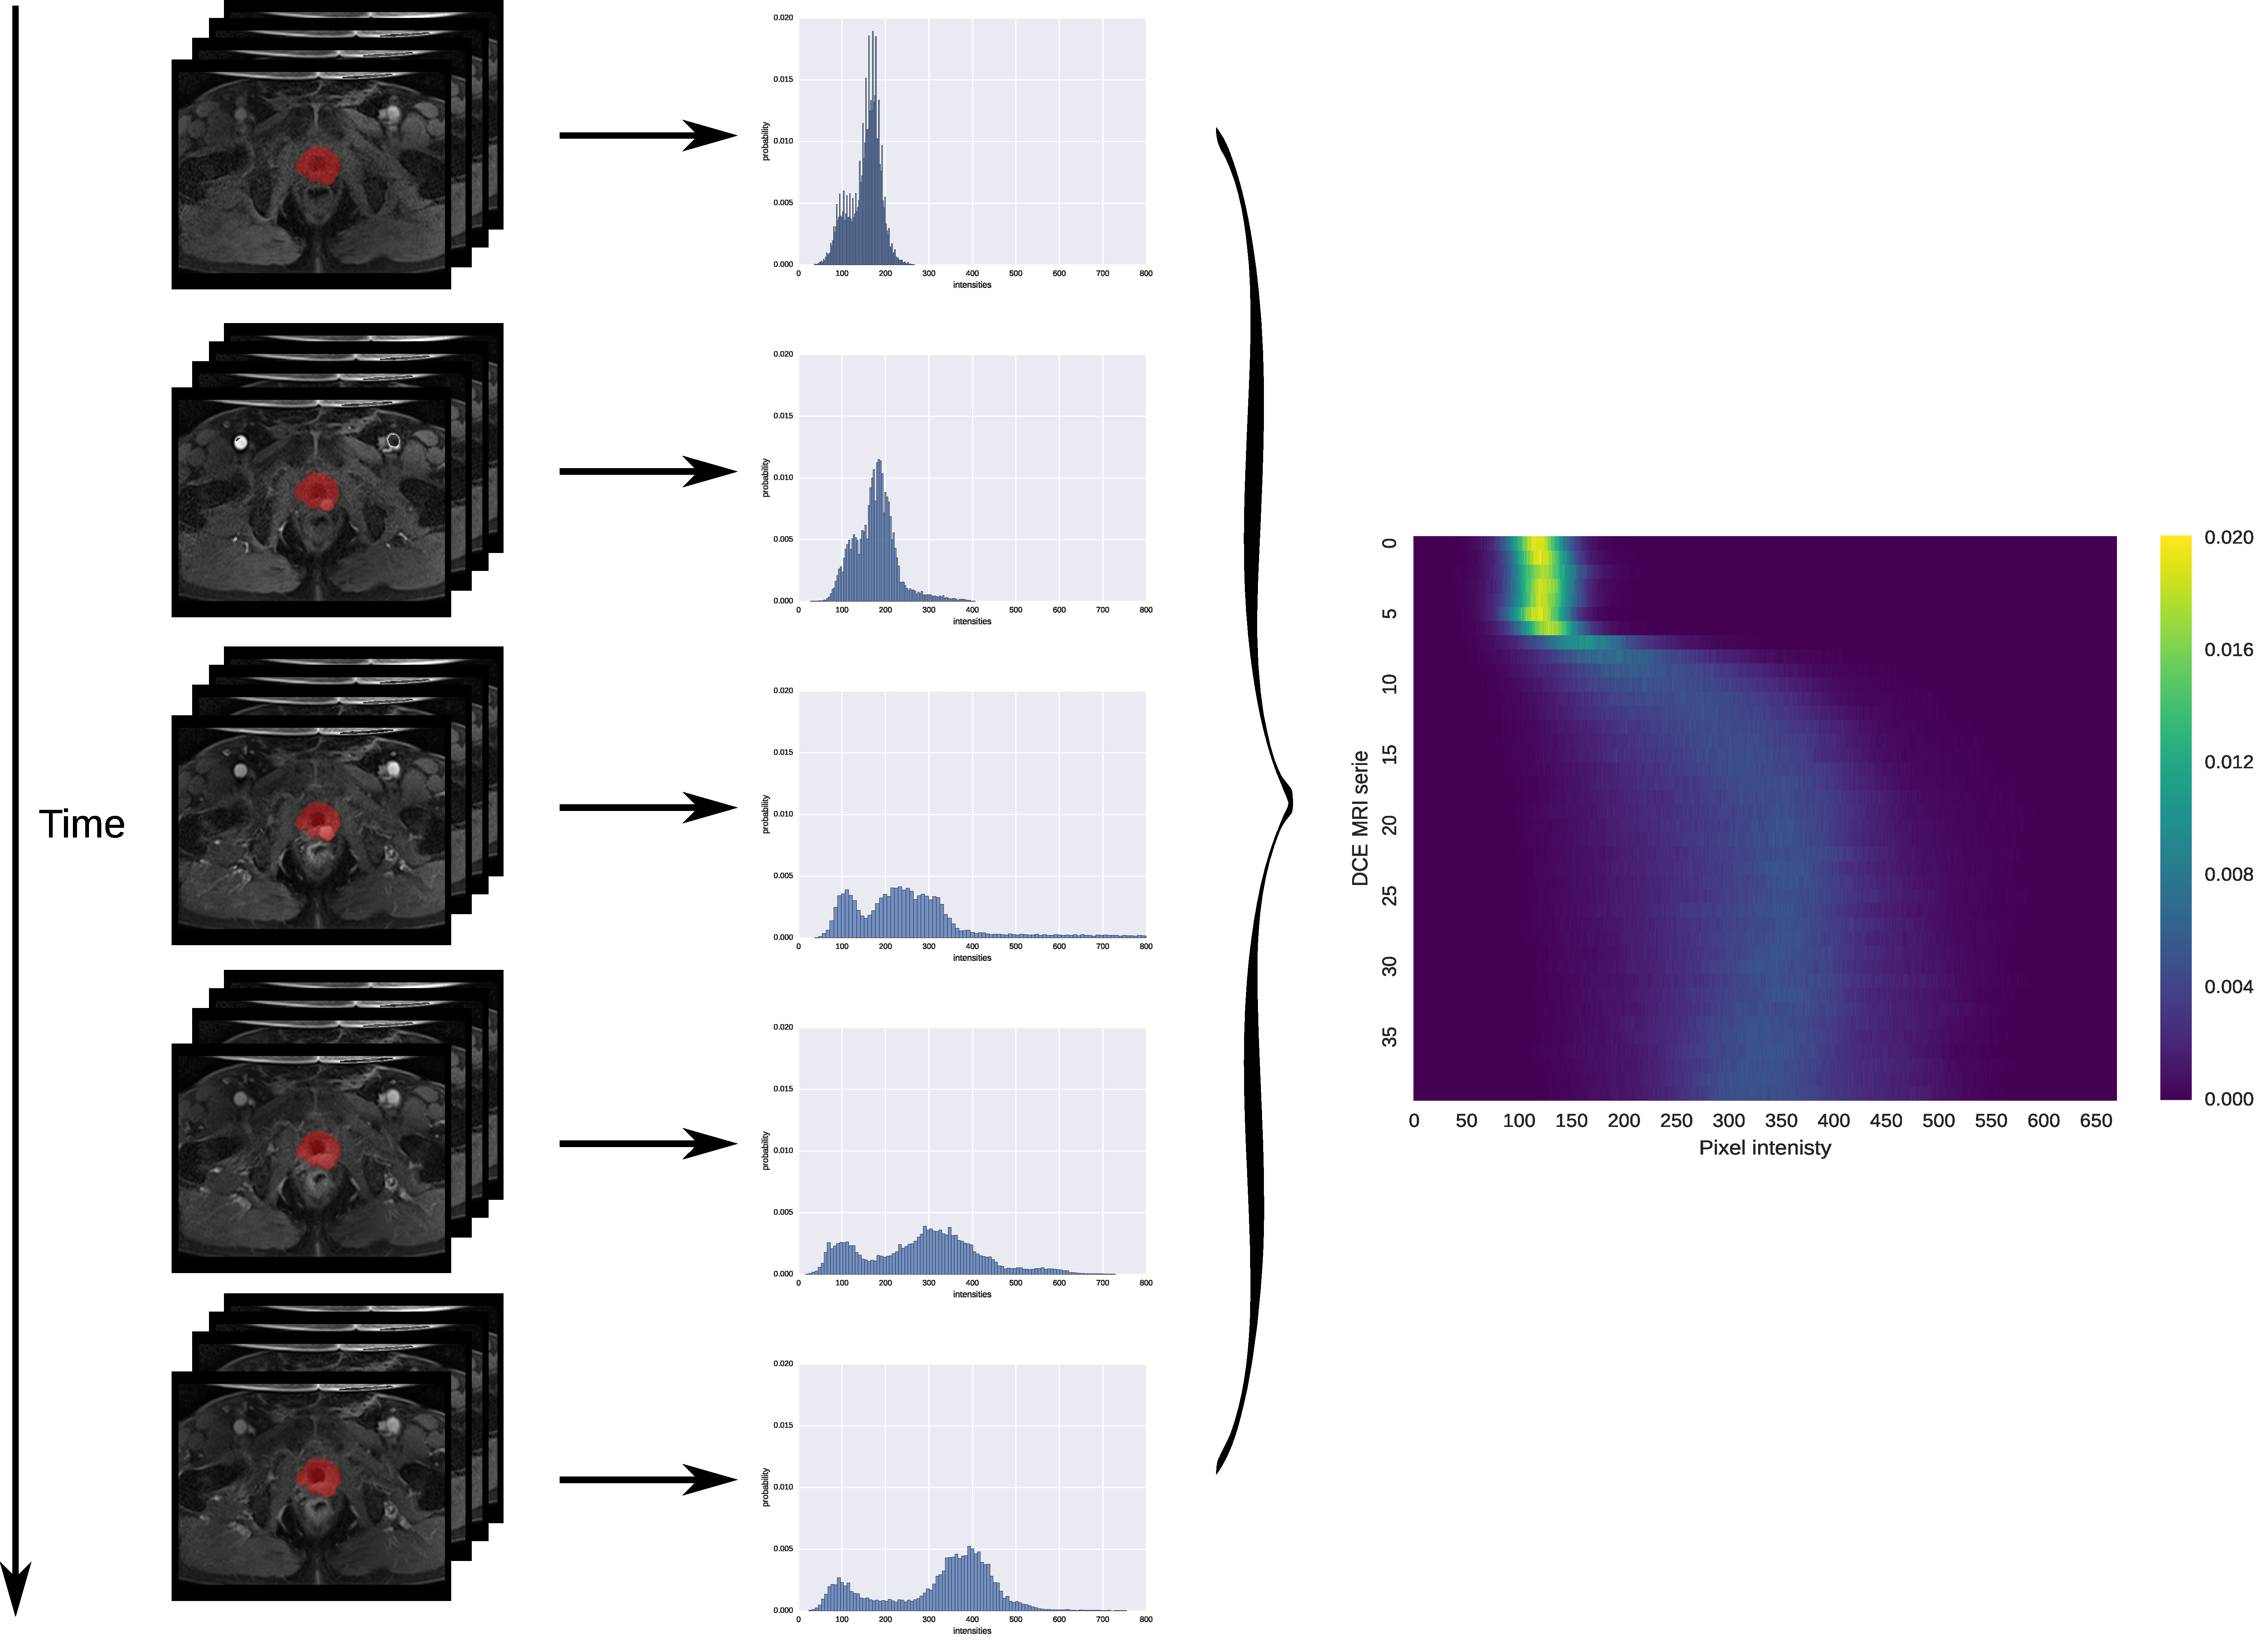
\includegraphics[width=1\textwidth]{02_methods/figures/heatmaprep.pdf}} \hfill
  \hspace*{\fill}
  \\
  \hspace*{\fill}
  \subfigure[]{\label{subfig:pat1}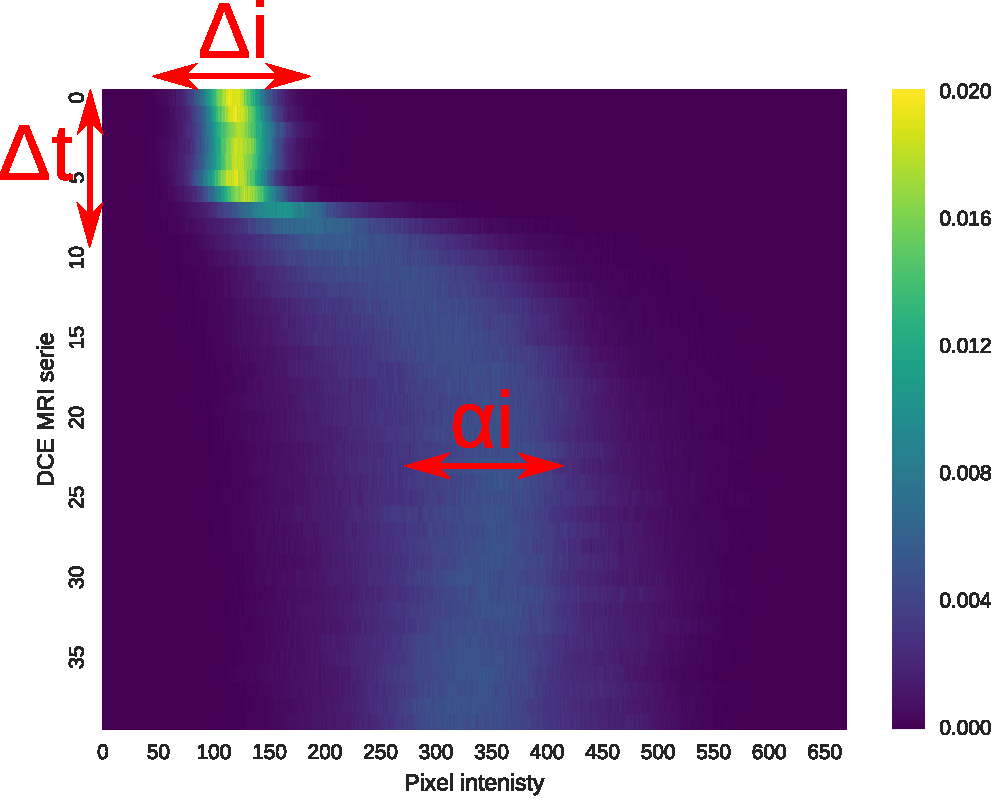
\includegraphics[width=.49\textwidth]{02_methods/figures/pat1_annotated.pdf}} \hfill
  \subfigure[]{\label{subfig:pat2}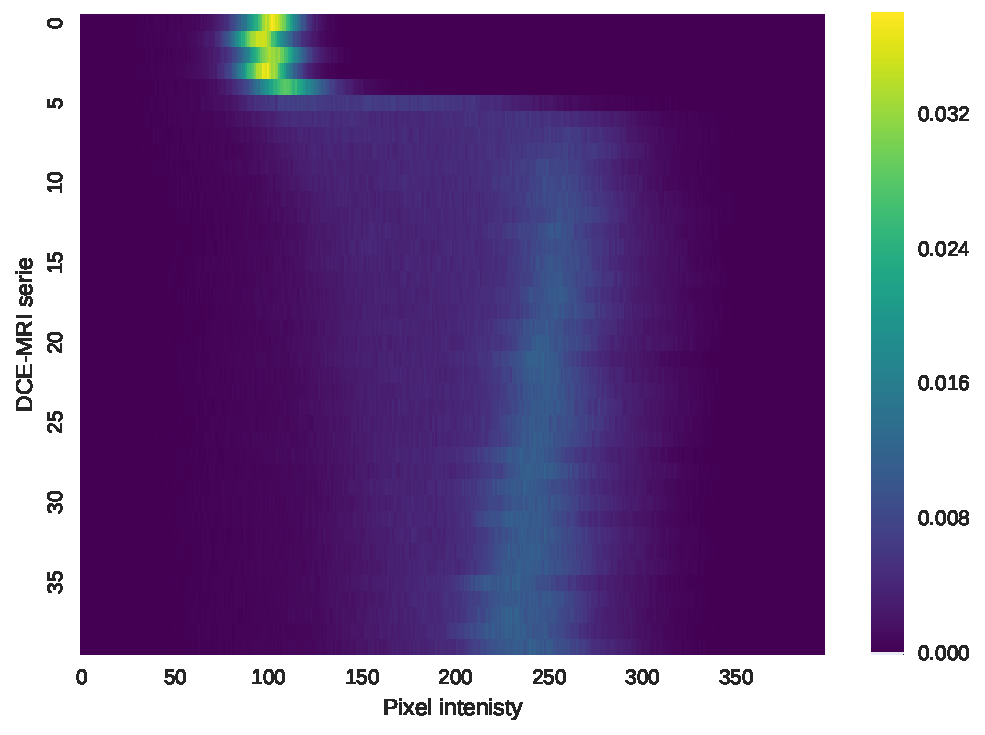
\includegraphics[width=.49\textwidth]{02_methods/figures/pat2.pdf}} \hfill
  \hspace*{\fill}
  \caption{\subref{subfig:pathhist} Illustration of the heatmap representation: all \ac*{pdf}s of the prostate gland are concatenated together to build an heatmap; \subref{subfig:pat1}-\subref{subfig:pat2} Illustration of inter-patient variations (i.e., $\Delta_i$, $\Delta_t$, and $\sigma_i$) \acs*{pdf} over time of two patients in a \ac{dce}-\ac{mri}.}
  \label{fig:heatmap}
\end{figure*}

In \ac{dce}-\ac{mri}, the intensity \ac{pdf} of prostate gland does not follow a unique type of distribution such as Rician or Gaussian distribution, as shown in Fig.\,\ref{subfig:pathist}.
Indeed, the inter-patient variations are more complex due to the temporal acquisition.
A better representation to observe these variations is to represent the intensity \ac{pdf} of the \ac{dce}-\ac{mri} data over time using a heatmap representation as shown in Fig.\,\ref{subfig:pathhist}.
Analyzing this heatmap representation across patients (see Fig.\,\ref{subfig:pat2}), the following variations are highlighted:
(i) an intensity offset $\Delta_i$ of the \ac{pdf} peak at pre-contrast,
(ii) a time offset $\Delta_t$ depending of the contrast agent arrival, and
(iii) a change of scale $\sigma_i$ related to the signal enhancement.
Therefore, our normalization method should attenuate all these variations and be performed globally across the different time sequence rather than for each independent sequence.

\subsubsection{Graph-based intensity offset correction}

\begin{figure}
  \centering
  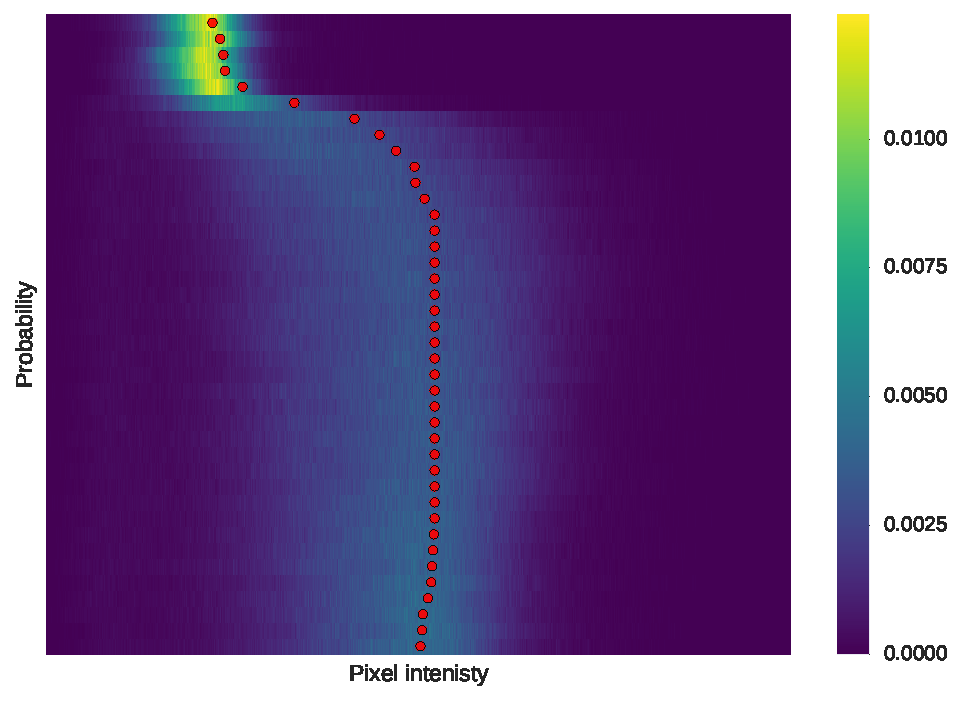
\includegraphics[width=0.7\linewidth]{02_methods/figures/estimator.pdf}
  \caption{Illustration of the estimator found using the shortest-path through the graph.}
  \label{fig:estimator}
\end{figure}

Before to standardize each sequence, the first step of the normalization is to cancel the intensity specific at each patient, occurring due to the media injection.
As previously mentioned, the intensity \ac{pdf} does not always follow either a Rician or a Gaussian distribution over time, in \ac{dce}-\ac{mri}.
Therefore, the mean of these distributions cannot be used as a potential estimate for these offsets.
Additionally, these offsets should be characterized by a smooth transition between series over time.
Thus, this problem is solved using the graph-theory: considering the intensity \ac{pdf} over time as shown in Fig.\,\ref{subfig:heatmaprep}, the offsets correspond to the boundary splitting the heatmap in two partitions such that they are as close as possible to the peak of the intensity \ac{pdf} (see Fig.\,\ref{fig:estimator} for an illustration).
Given the heatmap, a directed weighted graph $\mathcal{G}=(\mathcal{V}, \mathcal{E})$ is built by taking each bar--- i.e., the probability for a given time and pixel intensity---of the heatmap as a node and connecting each pair of bars by an edge.
The edge weight $w_{ij}$ between two nodes $i$ and $j$ corresponding to two pixels at position $(x_i, y_i)$ and $(x_j, y_j)$, respectively, is defined as in Eq.\,\eqref{eq:weight}:

\begin{equation}
  w_{ij} = \begin{cases}
    \alpha \exp(1 - \frac{H(i)}{\max(H)})       & \text{if } x_j = x_i + 1 \text{ and } y_j = y_i, \\
    (1 - \alpha) \exp(1 - \frac{H(i)}{\max(H)}) & \text{if } x_j = x_i \text{ and } y_j = y_i + 1, \\
    0                                           & \text{otherwise},
  \end{cases}
  \label{eq:weight}
\end{equation}

\noindent where $H$ is the heatmap, $\alpha$ is a smoothing parameter controlling the partitioning.

Therefore, these offsets are estimated by finding the shortest-path to cross the graph using Dijkstra's algorithm.
The entry and exiting nodes are set to be the bin with the maximum probability for the first \ac{dce}-\ac{mri} serie and the bin corresponding to the median value for the last \ac{dce}-\ac{mri} serie, respectively.
To ensure a robust estimation of these offsets, the process of finding the shortest-path is iteratively repeated by shifting the data and updating the heatmap as well as the graph $\mathcal{G}$.
The procedure is stopped once that the offset found does not change.
In general, this process is not repeated more than 3 iterations.
Figure~\ref{fig:estimator} illustrates the final estimation of the offsets (i.e., red landmark) found for each \ac{dce}-\ac{mri} serie.
Therefore, each intensity offset is subtracted for each \ac{dce}-\ac{mri}.

\subsubsection{Time offset and data dispersion correction}

\begin{figure*}
  \centering
  \hspace*{\fill}
  \subfigure[\acs*{rmse} computed for each patient of our dataset.]{\label{fig:rmse}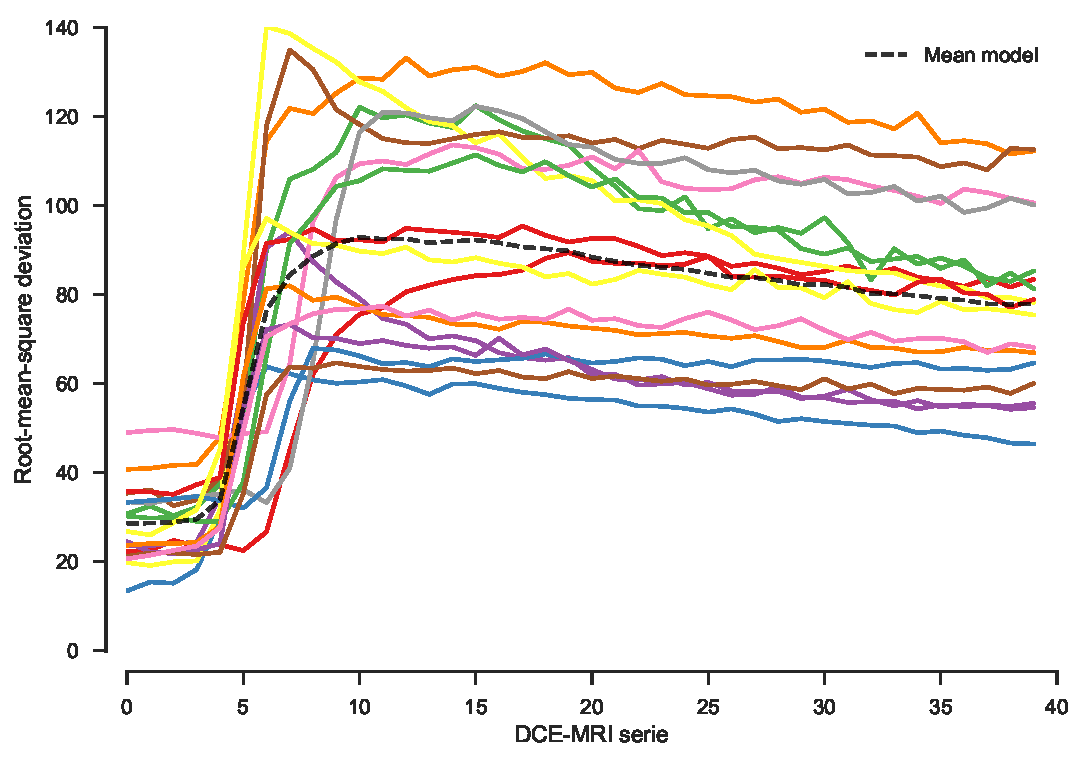
\includegraphics[width=.49\textwidth]{02_methods/figures/rmse.pdf}} \hfill
  \subfigure[\acs*{rmse} after alignment using the curve parametric model.]{\label{fig:rmseal}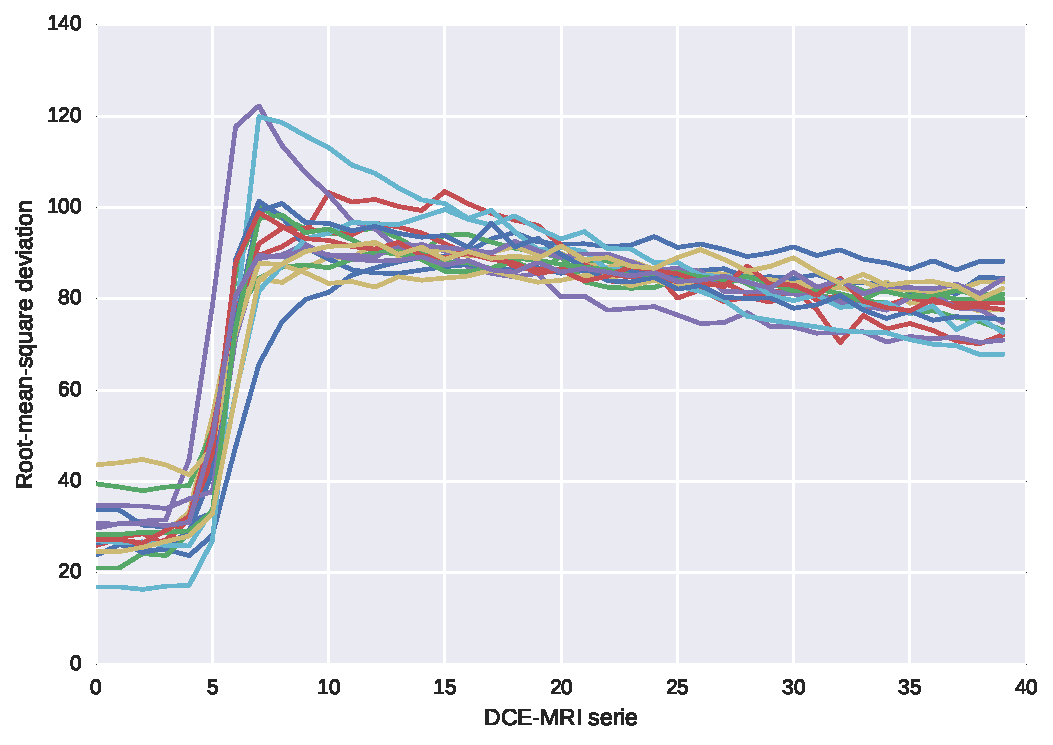
\includegraphics[width=.49\textwidth]{02_methods/figures/rmse_aligned.pdf}}
  \hspace*{\fill}
  \caption{Illustration of the correction of the time offset and the data dispersion.}
  \label{fig:curveal}
\end{figure*}

The next variations to correct are the time offset and the data dispersion.
By computing the \ac{rmse} of the intensities for each \ac{dce}-\ac{mri} serie, one can observe these two variations as shown in Fig.\,\ref{fig:rmse}.
Therefore, to correct these variations, we propose to register each patient \ac{rmse} to a mean model which corresponds to the mean of all patients \ac{rmse}.
The parametric model to perform the registration is formulated as in Eq.\,\eqref{eq:model}:

\begin{equation}
  T(\alpha, \tau, f(t)) = \alpha f(t - \tau) ,
  \label{eq:model}
\end{equation}

\noindent where $\alpha$ and $\tau$ are the two parameters handling the time offset and global scale, respectively, $f(\cdot)$ is the \ac{rmse} function define as:

\begin{equation}
  f(t) = \sqrt{ \left( \frac{\sum_{n=0}^{N} x(t)_{n}^2}{N}  \right) },
  \label{eq:rmsd}
\end{equation}

\noindent where $x(t)_n$ is the shifted intensity of a sample from a specific \ac{dce}-\ac{mri} serie at time $t$ from a total number of $N$ samples.

Therefore the registration problem is equivalent to:

\begin{equation}
  \argmin_{\alpha, \tau} = \sum_{t=0}^{N} \left[ T\left(\alpha, \tau, f(t)\right) - \mu(t) \right]^{2} ,
  \label{eq:cost}
\end{equation}

\noindent where $\mu(\cdot)$ is the mean model, $N$ is the number of \ac{dce}-\ac{mri} serie.

Illustration of the correction applied to each \ac{rmse} patient is shown in Fig.\,\ref{fig:rmseal}.
Once all these parameters have been inferred, the data can be shifted as well as scale.

\subsection{Quantification of \ac{dce}-\ac{mri}}\label{sec:stateart}

As stated in the introduction, one of our main challenge is to demonstrate the benefit of using our normalization method prior to extract parameters using quantitative and semi-quantitative methods.
In this section, we summarize the different methods which have been used for the quantification of \ac{dce}-\ac{mri} for \ac{cap} detection~\citep{lemaitre2015computer}.
Furthermore, we would like to emphasize the following additional contributions: (i) a novel automatic \ac{aif} estimation algorithm based on clustering and (ii) a simplified semi-quantitative method using constrained optimization.

\subsubsection{Brix and Hoffmann models}\label{sec:brixhoffmann}

In the Brix model~\citep{brix1991pharmacokinetic}, the \ac{mri} signal intensity is assumed to be proportional to the media concentration.
Therefore, the model is expressed as in Eq.\,\eqref{eq:brix}:

\begin{equation}
  s_n(t) = 1 + A \left[ \frac{\exp(k_{el} t') - 1}{k_{ep}(k_{ep} - k_{el})} \exp(- k_{el} t) - \frac{\exp(k_{ep} t') - 1}{k_{el}(k_{ep} - k_{el})} \exp(- k_{ep} t) \right],
  \label{eq:brix}
\end{equation}

\noindent with

\begin{equation}
  s_n(t) = \frac{s(t)}{S_0},
  \label{eq:enh}
\end{equation}

\noindent where $s(t)$ and $S_0$ are the \ac{mri} signal intensity at time $t$ and the average pre-contrast \ac{mri} signal intensity, respectively; $A$, $k_{el}$, and $k_{ep}$ are the constant proportional to the transfer constant, the diffusion rate constant, and the rate constant, respectively.
Additionally, $t'$ is set such that $0 \leq t \leq \tau$, $t' = t$ and afterwards while $t > \tau$, $t' = \tau$.

\citeauthor{hoffmann1995pharmacokinetic} proposed a similar model as expressed in Eq.\,\eqref{eq:hoffmann}, which derive from the Brix model:

\begin{equation}
  \small
  s_n(t) = 1 + \frac{A}{\tau} \left[ \frac{k_{ep} \left( \exp(k_{el} t') - 1 \right)}{k_{el}(k_{ep} - k_{el})} \exp(- k_{el} t) - \frac{\exp(k_{ep} t') - 1}{(k_{ep} - k_{el})} \exp(- k_{ep} t) \right] ,
  \label{eq:hoffmann}
\end{equation}

\noindent in which the constant $A$ is redefined by isolating the parameter $\tau$.

The parameters $A$, $k_{el}$, and $k_{ep}$ are estimated by fitting the model using non-linear least-squares optimization solved with Levenberg-Marcquardt.

\subsubsection{Tofts model}\label{sec:tofts}

The extended Tofts model is formulated as in Eq.\,\eqref{eq:exttofts}:

\begin{equation}
  C_t(t) = K_{trans} C_p(t) \Conv \exp(-k_{ep}t) + v_p C_p(t),
  \label{eq:exttofts}
\end{equation}

\noindent where $\Conv$ is the convolution operator; $C_t(t)$ and $C_p(t)$ is the concentration of contrast agent in the tissue and in the plasma, respectively; $K_{trans}$, $k_{ep}$, and $v_p$ are the volume transfer constant, the diffusion rate constant, and the plasma volume fraction, respectively.

Therefore, Tofts model requires to:
(i) detect candidate voxels from the femoral or iliac arteries and estimate a patient-based \ac{aif} signal,
(ii) convert the \ac{mri} signal intensity (i.e., \ac{aif} and dynamic signal) to a concentration, and
(iii) in the case of a population-based \ac{aif}, estimate an \ac{aif} signal.

\begin{figure*}
  \centering
  \hspace*{\fill}
  \subfigure[Original image.]{\label{fig:org}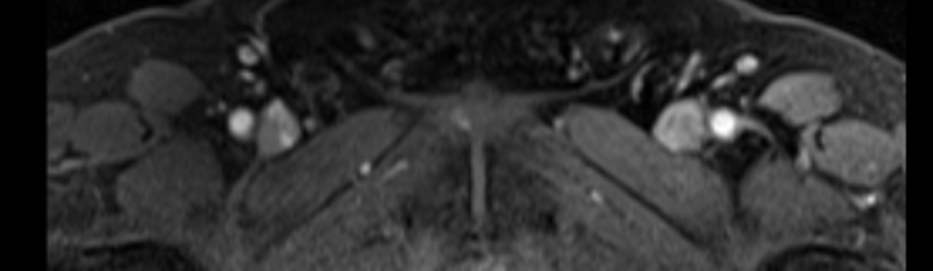
\includegraphics[width=.3\textwidth]{02_methods/figures/original.pdf}} \hfill
  \subfigure[Candidates region after clustering.]{\label{fig:cand}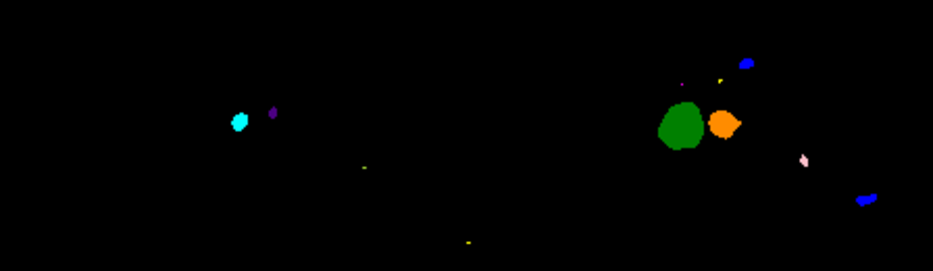
\includegraphics[width=.3\textwidth]{02_methods/figures/candidate.pdf}} \hfill
  \subfigure[Regions selected after applying the different criteria.]{\label{fig:final}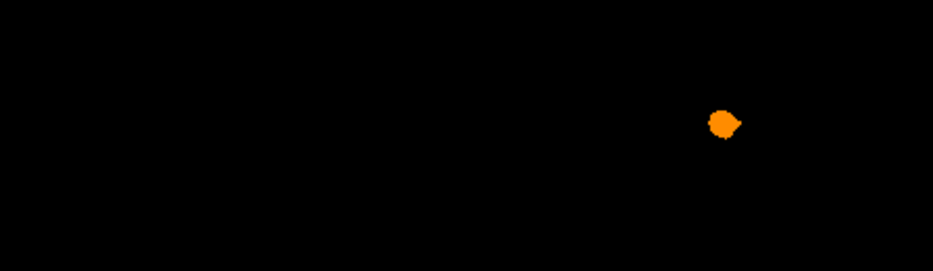
\includegraphics[width=.3\textwidth]{02_methods/figures/aif.pdf}}
  \hspace*{\fill}
  \caption{Illustration of the segmentation of the area used to determine the \acs*{aif}.}
  \label{fig:aif}
\end{figure*}

\begin{description}
  \item[Segmentation of artery voxels and patient-based \ac{aif} estimation] The \ac{aif} signal from \ac{dce}-\ac{mri} can be manually estimated by selecting the most-enhanced voxels from the femoral or iliac arteries~\citep{meng2010comparison}.
    Few methods have been proposed to address the automated extraction of \ac{aif} signal.
    \citeauthor{chen2008automatic} filtered successively the possible candidates to be considered as \ac{aif} such that~\citep{chen2008automatic}:
    (i) dynamic signals with small peak and voxels with a small wash-in are rejected by thresholding,
    (ii) a blob detector is used and large enough regions are kept, and
    (iii) circular and cylindricality criteria are used to reject the last false positive.
    \citeauthor{zhu2011automated} proposed an iterative method selecting voxels which best fit a gamma variate function~\citep{zhu2011automated}.
    However, it requires to compute first and second derivatives as well as maximum curvature points.
    \citeauthor{shanbhag2012generalized} proposed a 4-steps algorithm~\citep{shanbhag2012generalized,fennessy2015quantitative}:
    (i) remove slices with artefacts and find the best slices based on intrinsic anatomic landmarks and enhancement characteristics,
    (ii) find the voxel candidates using the maximum enhanced voxels and a multi-label maximum entropy based thresholding algorithm,
    (iii) exclude region next to the endorectal coil, and
    (iv) select the best 5 candidates which meet enhancement characteristics and that are correlated.

    All the above methods are rather complex and thus we propose a method which is based on the following simple assumptions:
    (i) all possible \ac{aif} signal candidates should have a similar shape,
    (ii) an high enhancement, and
    (iii) the arteries should be almost round and within a size range.
    Therefore, each slice is clustered into regions using K-means clustering with $k=6$.
    The cluster with the highest enhancement\textemdash i.e. corresponding to the 90\textsuperscript{th} percentile of the maximum of each dynamic signal\textemdash contain the arteries and is selected.
    Finally, regions with an eccentricity smaller than $0.5$ and an area in the range of $[100, 400]$ voxels are kept.
    Additionally, to remove voxels contaminated by partial volume effect, only the $10\%$ most enhanced voxels of the possible candidates are kept as proposed by~\citep{schabel2008uncertainty} and the average signal is computed.
    A summary of the different segmentation steps is presented in Fig.\,\ref{fig:aif}.
    \item[Conversion of \ac{mri} signal intensity to concentration] To estimate the free parameters of the Tofts model (see Eq.\,\eqref{eq:exttofts}), the concentration $C_t(t)$ and $C_p(t)$ need to be computed from the \ac{mri} signal intensity and the \ac{aif} signal, respectively.
      This conversion is based on the equation of the FLASH sequence\textemdash see~\ref{app:signaltoconc} for details\textemdash and is formulated as in Eq.\,\eqref{eq:conv}:
      \begin{equation}
        c(t) = \frac{1}{TR \cdot r_1} \ln\left( \frac{1 - \cos \alpha \cdot S^{*}\frac{s(t)}{S_0}}{1 - S^{*}\frac{s(t)}{S_0}} \right) - \frac{R_{10}}{r_1} ,
        \label{eq:conv}
      \end{equation}
      \noindent with,
      \begin{equation}
        S^{*} = \frac{1 - \exp(- TR \cdot R_{10})}{1 - \cos \alpha \cdot \exp(- TR \cdot R_{10})} ,
        \label{eq:sstarconv}
      \end{equation}
      \noindent where $s(t)$ is the \ac{mri} signal, $S_0$ is the \ac{mri} signal prior to the injection of the contrast media, $\alpha$ is the flip angle, $TR$ is the \acf{tr}, $R_{10}$ is the pre-contrast tissue relaxation time also equal to $\frac{1}{T_{10}}$, $r_1$ is the relaxitivity coefficient of the contrast agent.

      $T_{10}$ can be estimated from the acquisition of a T$_1$ map.
      However, this modality is not part of the clinical trial in this research and the value of $T_{10}$ is fixed to \SI{1600}{\ms} for both blood and prostate, in accordance with the values found in the literature~\citep{fennessy2015quantitative,de2004mr,carr2011magnetic}.
      \item[Estimation of population-based \ac{aif}] While estimating the pharmacokinetic parameters from Tofts model, the \ac{aif} concentration $C_p(t)$ can be computed either from the patient or a population.
        We presented in the two previous sections the algorithms which allows to estimate the patient-based \ac{aif} concentration.
        To compare with the previous approach, we also computed a population-based \ac{aif} which will be also used later to compare the performance of both approaches.
        In that regard, the population-based \ac{aif} was estimated as in~\citep{meng2010comparison} by fitting the average patient-based \ac{aif}s to the model of~\cite{parker2006experimentally} which is formulated as in Eq.\,\eqref{eq:parker}:
        \begin{equation}
          C_p(t) = \sum_{n=1}^{2} \frac{A_n}{\sigma_n \sqrt{2 \pi}} \exp\left(\frac{- (t- T_n)^2}{2\sigma_{n}^{2}}\right) + \frac{\alpha \exp(-\beta t)}{1 + \exp{-s (t - \tau)}} ,
          \label{eq:parker}
        \end{equation}
        \noindent where $A_n$, $T_n$, and $\sigma_n$ are the scaling constants, centers, and widths of the n\textsuperscript{th} Gaussian, $\alpha$ and $\beta$ are the amplitude and decay constant of the exponential; and $s$ and $\tau$ are the width and center of the sigmoid function, respectively.
\end{description}

The parameters are estimated by fitting the model using non-linear least-squares optimization solved with Levenberg-Marcquardt.

\subsubsection{\acs*{pun} model}\label{sec:pun}

\citeauthor{gliozzi2011phenomenological} showed that \ac{pun} approach can be used for \ac{dce}-\ac{mri} analysis~\citep{gliozzi2011phenomenological}.
The model has been successfully used in a \ac{cad} system proposed by~\cite{giannini2015fully}.
This model can be expressed as in Eq.\,\eqref{eq:pun}:

\begin{equation}
  s_n(t) = \exp\left[rt + \frac{1}{\beta} \left( a_0 - r \right) \left( \exp(\beta t) - 1 \right) \right],
  \label{eq:pun}
\end{equation}

\noindent with

\begin{equation}
  s_n(t) = \frac{s(t) - S_0}{S_0},
  \label{eq:enh}
\end{equation}

\noindent where $s(t)$ and $S_0$ are the \ac{mri} signal intensity at time $t$ and the average pre-contrast \ac{mri} signal intensity, respectively; $r$, $a_0$, and $\beta$ are the free parameters of the model.

The parameters are estimated by fitting the model using non-linear least-squares optimization solved with Levenberg-Marcquardt.

\subsubsection{Semi-quantitative analysis}\label{sec:semi}

The semi-quantitative analysis of the \ac{dce}-\ac{mri} is equivalent to extracting curve characteristics directly from the signal without a strict theoretical pharmacokinetic meaning.
In this work, we use the model presented by~\cite{huisman2001accurate} which formulated the \ac{mri} signal as in Eq.\,\eqref{eq:huisman}:

\begin{equation}
  s(t) = \begin{cases}
    S_0 & 0 \leq t \leq t_0 \\
    S_M - (S_M - S_0) \exp\left( \frac{-(t - t_0)}{\tau} \right) & t_0 < t \leq t_0 + 2 \tau \\
    S_M - (S_M - S_0) \exp\left( \frac{-(t - t_0)}{\tau} \right) + w(t - t_0 + 2 \tau) & t > t_0 + 2 \tau
  \end{cases}
  \label{eq:huisman}
\end{equation}

\noindent where $s(t)$ is the \ac{mri} signal intensity, $S_0$ is the pre-contrast signal intensity, $t_0$ is the time corresponding to the start of enhancement, $S_M$ and $\tau$ is the maximum of the signal and the exponential time constant, and $w$ is the slope of the linear part.

\citeauthor{huisman2001accurate} argue that curve fitting via least-squares minimization using Nelder-Mead algorithm leads to inaccurate estimation of the free parameters: mainly the issue come from an incorrect estimation of the start of enhancement $t_0$ leading to incorrect estimation of the other parameters.
Therefore, they propose to:
(i) estimate robustly $t_0$,
(ii) estimate $S_0$ by averaging the samples between $0$ and $t_0$
(ii) estimate $w$ depending if the slope is significant or not,
(iii) estimate $S_M$ which should be the point at the intersection of the most probable slope line and the plateau.

Instead of these successive estimations, we propose a unified optimization in which $t_0$ is fixed since that this is a key parameter.
Therefore, $t_0$ is robustly estimated from the \ac{aif} signal since that this is the most enhanced signal in which the start of enhancement is easily identifiable.
The \ac{aif} signal is computed as in Section~\ref{sec:tofts}.
$t_0$ is estimated by finding the maximum of the first derivative of the \ac{aif} signal, always occurring at the beginning of the signal.
Then, the function in Eq.\,\eqref{eq:huisman} is fitted using non-linear least squares with Trust Region Reflective algorithm~\citep{sorensen1982newton}.
Furthermore, the parameters $\tau$ and $S_M$ are bounded during the optimization to ensure robust estimations.
$\tau$ is bounded between $t_0$ and $t_f$ which is the time of the last sample while $S_M$ is bounded between $S_0$ and $\max(s(t))$.


From Eq.\,\eqref{eq:huisman}, the following features are extracted:
(i) the wash-in corresponding to the slope between $t_0$ and $t_0 + 2 \tau$,
(ii) the wash-out corresponding to the parameter $w$,
(iii) the area under the curve between $t_0$ and the end of the signal,
(iv) the exponential time constant $\tau$, and
(v) the relative enhancement $S_M - S_0$.

%%% Local Variables: 
%%% mode: latex
%%% TeX-master: "../main"
%%% End: 

\section{Materials}\label{sec:materials}

\subsection{Data}\label{sec:data}

The multi-parametric \ac{mri} data are acquired from a cohort of patients with higher-than-normal level of \ac{psa}.
The acquisition is performed using a 3T whole body \ac{mri} scanner (Siemens Magnetom Trio TIM, Erlangen, Germany) using sequences to obtain \ac{t2w}-\ac{mri}, \ac{dce}-\ac{mri} and \ac{dw}-\ac{mri}.
Aside of the \ac{mri} examination, these patients also have underwent a guided-biopsy.
The dataset is composed of a total of 20 patients of which 18 patients have biopsy proven \ac{cap} and 2 patients are ``healthy'' with negative biopsies.
Therefore, 13 patients have a \ac{cap} in the \ac{pz}, 3 patients have \ac{cap} in the \ac{cg}, 2 patients have invasive \ac{cap} in both \ac{pz} and \ac{cg} and finally 2 patients are considered as ``healthy''.
An experienced radiologist has segmented the prostate organ --- on \ac{t2w}-\ac{mri} and \ac{dce}-\ac{mri} --- as well as the prostate zones (i.e., \ac{pz} and \ac{cg}) and \ac{cap} on the \ac{t2w}-\ac{mri}.

A \SI{3}{\mm} slice fat-suppressed \ac{t2w} fast spin-echo sequence (\ac{tr}/\ac{te}/\ac{etl}: \SI{3400}{\ms}/\SI{85}{\ms}/13) is used to acquire images in sagittal and oblique coronal planes, the latter planes being orientated perpendicular or parallel to the prostate \ac{pz} – rectal wall axis.
Three-dimensional \ac{t2w} fast spin-echo (\ac{tr}/\ac{te}/\ac{etl}: \SI{3600}{\ms}/\SI{143}{\ms}/109, slice thickness: \SI{1.25}{\mm}) images are then acquired in an oblique axial plane.
The nominal matrix and \ac{fov} of the 3D \ac{t2w} fast spin-echo images are $320 \times 256$ and $280 \times 240$ mm\textsuperscript{2}, respectively, thereby affording sub-millimetric pixel resolution within the imaging plane.

\ac{dce}-\ac{mri} is performed using a fat suppressed 3D T$_1$ VIBE sequence (\ac{tr}/\ac{te}/Flip angle: \SI{3.25}{\ms}/\SI{1.12}{\ms}/\SI{10}{\degree}; Matrix: $256 \times 192$; \ac{fov}: $280 \times 210$ (with 75\% rectangular \ac{fov}); slab of 16 partitions of \SI{3.5}{\mm} thickness; temporal resolution: \SI{6}{\s}/slab over approximately \SI{5}{\minute}).
A power injector (Medrad, Indianola, USA) is used to provide a bolus injection of Gd-DTPA (Dotarem, Guerbet, Roissy, France) at a dose of \SI{0.2}{\ml} Gd-DTPA/kg of body weight.

These \ac{dce}-\ac{mri} sequences are resampled using the spatial information of the \ac{t2w}-\ac{mri} and missing data are interpolated using a linear interpolation.
The volumes of the \ac{dce}-\ac{mri} dynamic are rigidly registered, to remove any patient motion during the acquisition.
Furthermore, a non-rigid registration is performed between the \ac{t2w}-\ac{mri} and \ac{dce}-\ac{mri} in order to propagate the prostate zones and \ac{cap} ground-truths.
The resampling is implemented in C++ using the Insight Segmentation and Registration Toolkit~\citep{ibanez2005itk}.

\subsection{Implementation}

The implementation of the registration (C++), normalization (Python), and classification pipeline (Python) are publicly available on GitHub\footnote{\url{https://github.com/I2Cvb/lemaitre-2016-nov/tree/master}}.
The data used for this work are also publicly available\footnote{\url{https://zenodo.org/record/61163}}.

\section{Experiments and results}\label{sec:experiments}

\subsection{Goodness of model fitting}\label{sec:fit}

%{\color{red} In case that we have issue with $R^2$, we need to provide the AIC since that the model are usually non-linear.}

\begin{table*}
  \caption{Coefficient of determination $R^{2}$ (i.e., $\mu \ (\pm \sigma)$), while fitting data with the different quantification models.}
  \centering
  \resizebox{\columnwidth}{!}{
  \begin{tabular}{lc c c c c c}
    \toprule
    Data type & Brix & Hoffmann & Tofts population \ac{aif} & Tofts patient \ac{aif} & \ac{pun} & Semi-quantitative \\
    \midrule
    Un-normalized & $0.85 \ (\pm 0.11)$ & $0.81 \ (\pm 0.17)$ & $0.84 \ (\pm 0.14)$ & $0.88 \ (\pm 0.12)$ & $0.27 \ (\pm 0.18)$ & $0.64 \ (\pm 0.24)$  \\
    Normalized    & $0.92 \ (\pm 0.05)$ & $0.72 \ (\pm 0.32)$ & $0.92 \ (\pm 0.06)$ & $0.90 \ (\pm 0.10)$ & $0.28 \ (\pm 0.20)$ & $0.75 \ (\pm 0.20)$  \\
    \bottomrule
  \end{tabular}
  }
  \label{tab:r2}
\end{table*}

Parameter estimation of the quantification methods are related to fit a specific model to the \ac{dce}-\ac{mri} data.
Therefore, this section report the goodness of fitting by computing the coefficient of determination $R^2$ such as in Eq.\,\eqref{eq:r2}

\begin{equation}
  R^2 = 1 - \frac{\sum_{t = 1}^{T} (s_t - \hat{s}_t)^2}{\sum_{t = 1}^{T} (s_t - \bar{s})^2} ,
  \label{eq:r2}
\end{equation}

\noindent where $s_t$ and $\hat{s}_t$ are the signal to be fitted and the estimated signal at time $t$, respectively; $\bar{s}$ is the average signal to be fitted.

Mean and standard-deviation of the coefficient of determination $R^{2}$ is reported in Table~\ref{tab:r2} for each quantification model.
Brix, Hoffmann, and Tofts models are fitted with a coefficient $R^{2}$ superior to 0.80.
Additionally, the proposed \ac{pun} model does not seem to fit well the data.
Normalizing the data improve the coefficient $R^2$ for all the methods apart of the Hoffmann model.
The large standard deviation for this model might imply that there is some cases, that the fitting fails.

\subsection{Detection of \acs*{cap} using pharmacokinetic parameters}

\begin{table*}
  \caption{\acs*{auc} for each individual pharmacokinetic parameter using a \acs*{rf} classifier.}
  \centering
  \resizebox{\columnwidth}{!}{
  \begin{tabular}{l c c}
    \toprule
    \textbf{Features} & Un-normalized data & Normalized data \\
    \midrule
    \textbf{Brix model} & & \\
    \quad $A$         & 0.54 & 0.55 \\
    \quad $k_{el}$    & 0.51 & 0.50 \\
    \quad $k_{ep}$    & 0.55 & 0.58 \\
    \textbf{Hoffmann model} & & \\
    \quad $A$         & 0.52 & 0.51 \\
    \quad $k_{el}$    & 0.55 & 0.53 \\
    \quad $k_{ep}$    & 0.55 & 0.54 \\
    \textbf{Tofts model with population \ac{aif}} & & \\
    \quad $K_{trans}$ & 0.56 & 0.55 \\
    \quad $k_{ep}$     & 0.49 & 0.49 \\
    \quad $v_{p}$     & 0.53 & 0.50 \\
    \textbf{Tofts model with patient \ac{aif}} & & \\
    \quad $K_{trans}$ & 0.57 & 0.57 \\
    \quad $k_{ep}$     & 0.51 & 0.53 \\
    \quad $v_{p}$     & 0.53 & 0.55 \\
    \textbf{\ac{pun} model} & & \\
    \quad $a_0$       & 0.52 & 0.53 \\
    \quad $r$         & 0.55 & 0.57 \\
    \quad $\beta$     & 0.53 & 0.55 \\
    \textbf{Semi-quantitative analysis} & & \\
    \quad wash-in     & 0.57 & 0.53 \\
    \quad wash-out    & 0.52 & 0.49 \\
    \quad IAUC        & 0.51 & 0.51 \\
    \quad $\tau$      & 0.57 & 0.54 \\
    \quad $S_M - S_0$ & 0.56 & 0.53 \\
    \bottomrule
  \end{tabular}
  }
  \label{tab:resfeats}
\end{table*}

\begin{figure*}
  \centering
  \hspace*{\fill}
  \subfigure[Without normalization.]{\label{fig:rfpharmaunorm}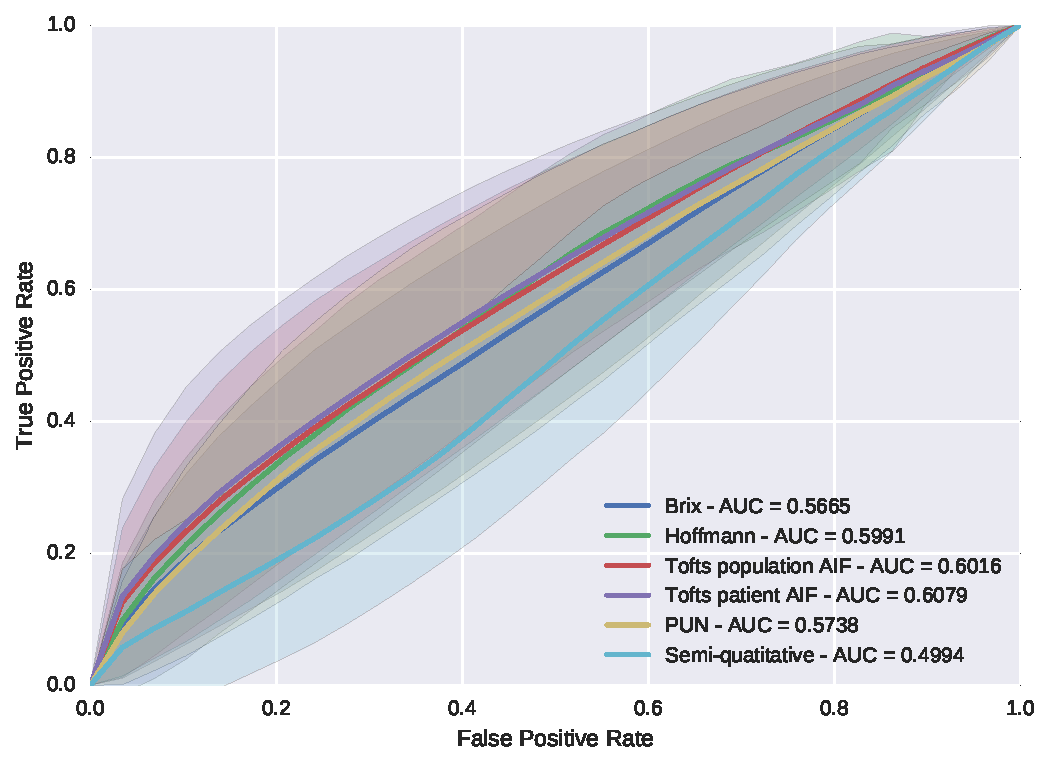
\includegraphics[width=.49\textwidth]{03_experiments/figures/unormalized/rf.pdf}} \hfill
  \subfigure[With normalization.]{\label{fig:rfpharmanorm}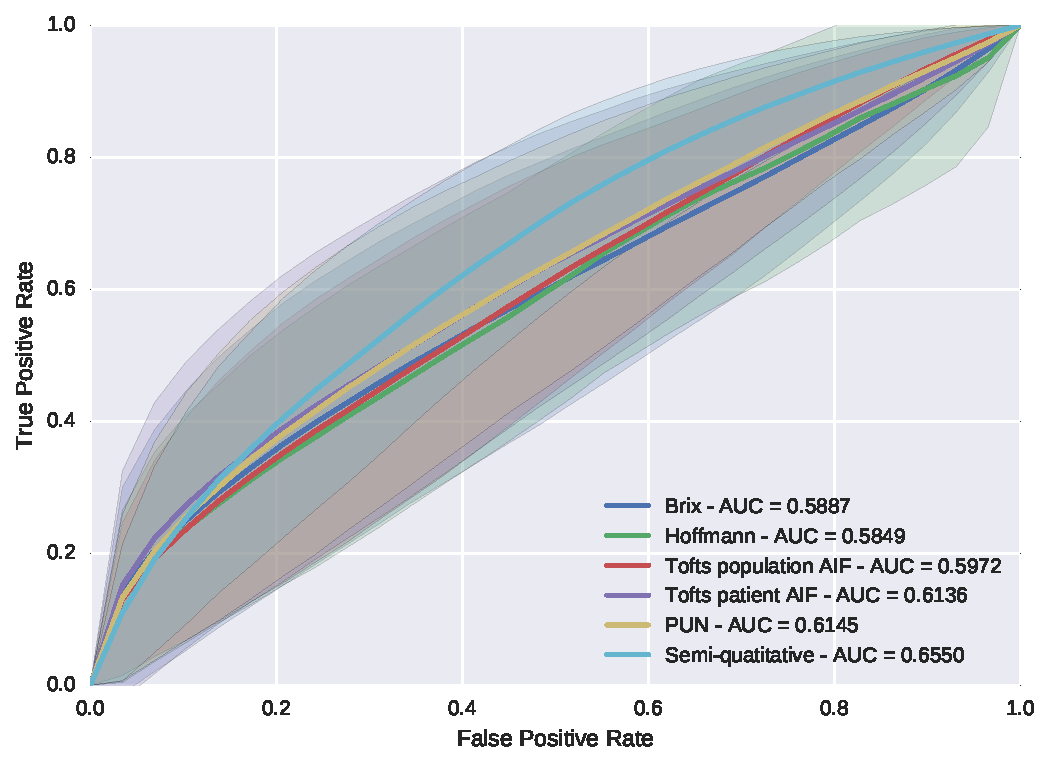
\includegraphics[width=.49\textwidth]{03_experiments/figures/normalized/rf.pdf}}
  \hspace*{\fill}
  \caption{\acs*{roc} analysis using a \acs*{rf} classifier with and without normalization \ac{dce}-\ac{mri} data for different pharmacokinetic models.}
  \label{fig:normpharmarf}
\end{figure*}

To study the potential benefit of our normalization, \ac{cap} are detected using pharmacokinetic parameters estimated from un-normalized and normalized \ac{dce}-\ac{mri} data.
Each individual pharmacokinetic parameter is classified to evaluate their individual discriminative power to detect \ac{cap}.
Therefore, a \ac{rf} classifier is used in conjunction with a \ac{lopo}.
The use of \ac{rf} is motivated since that it leads to the best performance in the state-of-the-art methods~\citep{litjens2014computer,lemaitre2015computer}.
Results are summarized in Table~\ref{tab:resfeats} in terms of \ac{auc}.
Normalization can improve the detection of \ac{cap}; however, the benefit of normalization is more obvious by combining the pharmacokinetic features of each model, as previously done in traditional \ac{cad} system~\citep{lemaitre2015computer}.
For the latter configuration, results are summarized by performing a \ac{roc} analysis and computing the \ac{auc}, as reported in Fig.\,\ref{fig:normpharmarf}.
Quantification using normalized data outperforms quantification using un-normalized data in terms of classification performance apart of Hoffmann and Tofts population-based \ac{aif} models.
The reasons behind the decrease of the \ac{auc} might be related to: (i) a poor fitting as discussed in Sect.\,\ref{sec:fit} (cf., Hoffmann model) and (ii) a small number of patient while estimating some parameters (cf., Tofts model).
The best classification performance are obtained using the semi-quantitative approach with an \ac{auc} of 0.655.

\subsection{Classification of the entire enhanced \acs*{dce}-\acs*{mri} signal}

\begin{figure}
  \centering
  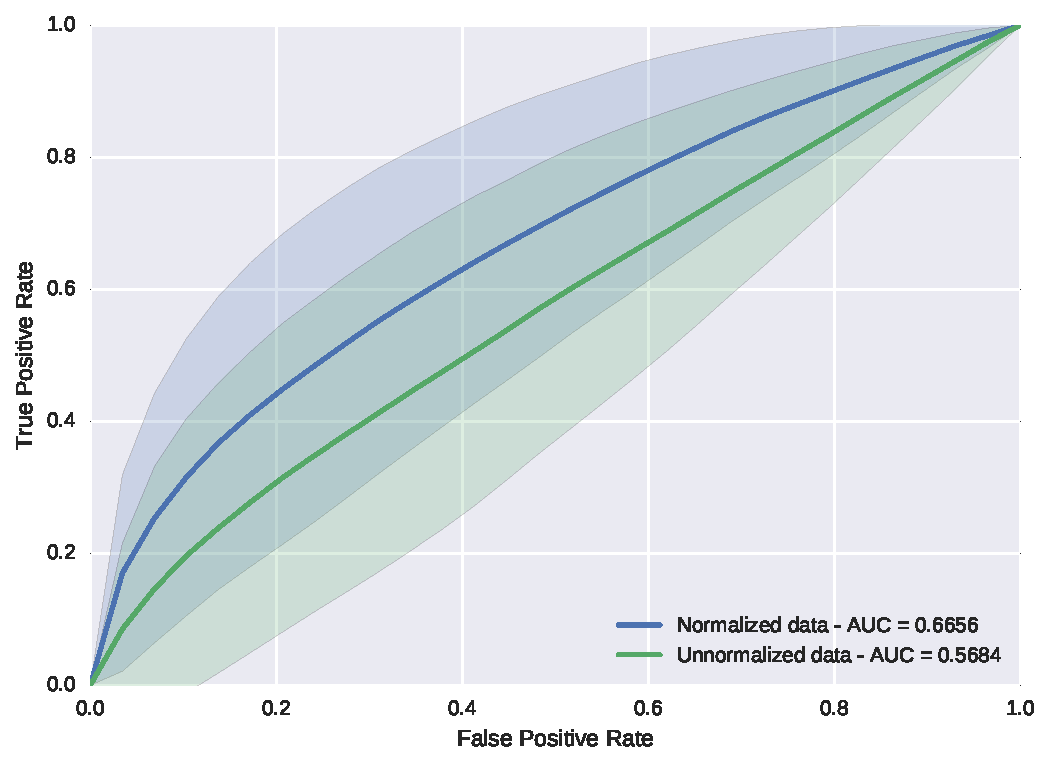
\includegraphics[width=0.7\linewidth]{03_experiments/figures/rf.pdf}
  \caption{\acs*{roc} analysis using the entire \ac{dce}-\ac{mri} signal with and without normalization in conjunction with a \acs*{rf} classifier.}
  \label{fig:rfnormdcesignal}
\end{figure}

As stated in the introduction, the quantification methods are extracting a set of parameters characterizing the enhancement \ac{dce}-\ac{mri} signal.
However, this extraction might lead to a loss of information.
This experiment is performed to assess if making use of the whole \ac{dce}-\ac{mri} signal instead of the just the pharmacokinetic parameters can improve the classification performance.
Therefore, each enhanced \ac{dce}-\ac{mri} signal, normalized and un-normalized, is classified using a \ac{rf} classifier in a \ac{lopo} fashion.
The \ac{roc} analysis and \ac{auc} are reported in Fig.\,\ref{fig:rfnormdcesignal}.
Classification without normalization lead to the worst performance, with an \ac{auc} of 0.568.
However, data normalization in conjunction with the use of the whole \ac{dce}-\ac{mri} signal is the strategy which outperforms all others, with an \ac{auc} of 0.666.

%%% Local Variables: 
%%% mode: latex
%%% TeX-master: "../main"
%%% End: 

\section{Discussions}\label{sec:discussions}

The experiments conducted in the previous section can incite several discussions.
In Tofts quantification, two different approaches have been used to infer the pharmacokinetic parameters: using a population-based or a patient-based \ac{aif}.
The patient-based \ac{aif} approach leads to better classification performance.
However, there are two shortcomings to take into account when considering this fact:
(i) the T$_{10}$ parameter has been fixed and is not computed from a T$_1$ map and
(ii) the population-based \ac{aif} has been estimated from a cohort of only 17 patients.
These two limitations have to be considered when asserting that
population-based \ac{aif} modeling outperforms patient-based \ac{aif} modeling.

The best classification performance is achieved by normalizing the
\ac{dce}-\ac{mri} data and using the entire enhanced signal as a
feature, emphasizing the fact that a \emph{loss of information} may occur while extracting quantitative parameters.
Furthermore, normalization is a less complex process than all
quantification methods and significantly improves the classification
performance of the semi-quantitative approach ($p=0.001$) proposed by
\citeauthor{huisman2001accurate}.
Additionally, our normalization improves the \ac{auc} score related to
the detection of \ac{cap} in \ac{cg}, also known to be the most
challenging cases in the diagnosis of \ac{cap}.

However, using the entire enhanced signal in conjunction with the
normalization is limited by one drawback: the training time of the
\ac{rf} classifier increases; instead of using $3$ to $5$ features, so the
feature space becomes a $40$ dimensional space. The extraction of the
semi-quantitative parameters leads to a comparable classification performance ---
$0.655 \pm 0.108$ vs. $0.666 \pm 0.154$ --- and should be chosen as the alternative method to
consider if the number of feature in the classification is
critical. Despite this fact, the benefit of our proposed normalization method
has been shown for both methods.

Nevertheless, this study is performed on a small cohort of patients using a single \ac{mri} machine.
Generalizing the results of this study onto a larger dataset acquired
from different commercial systems needs to be considered to study the robustness of the proposed approach.
Additionally, our method being non-parametric should provide an
adequate framework to process \ac{dce} data from different
institutions, scanners with different settings.

%%% Local Variables:
%%% mode: latex
%%% TeX-master: "../main"
%%% End:

\section{Conclusions and future works}\label{sec:conclusions}

In this work, we presented a new method for normalizing/standardizing \ac{dce}-\ac{mri} data.
This method aimed at reducing the inter-patient variations occurring during data acquisition.
A graph-based approach was used to correct intensity offset in conjunction with a model-based correction to reduce time offset as well as intensity scaling.
We show the benefit of our normalization method prior to extract quantitative and semi-quantitative features, with a significant improvement of the classification performance.
Nevertheless, we also show that using the whole normalized \ac{dce}-\ac{mri} signal outperforms all quantitative approaches.

As avenues for future research, this normalization has to be part of a \ac{mpmri} \ac{cad} system in which \ac{dce}-\ac{mri} modality needs to be combined with other complementary modalities.

%%% Local Variables: 
%%% mode: latex
%%% TeX-master: "../main"
%%% End: 

\appendix
\section{Conversion from FLASH signal to media concentration}\label{app:signaltoconc}

In this appendix, we show the demonstration used to extract the agent concentration from the \ac{mri} signal.

The signal equation in FLASH sequence~\citep{haase1986flash} is defined as:

\begin{equation}
  s(t) = S_{eq} \sin \alpha \cdot \frac{1 - \exp\left(-TR\left(R_{10} + r_1 c(t)\right)\right)}{1 - \cos \alpha \cdot \exp\left(-TR\left(R_{10} + r_1 c(t)\right)\right)} ,
  \label{eq:app:flash}
\end{equation}

\noindent where $s(t)$ is the \ac{mri} signal, $S_{eq}$ is the maximum signal amplitude of the spoiled gradient at the \ac{te} which is proportional to the \ac{pd}, $\alpha$ is the flip angle, $TR$ is the \acf{tr}, $R_{10}$ is the pre-contrast tissue relaxation time also equal to $\frac{1}{T_{10}}$, $r_1$ is the relaxitivity coefficient of the contrast agent, and $c(t)$ is the media concentration.

Therefore, the pre-contrast signal prior to bolus injection of the media is defined as:

\begin{equation}
  S_0 = S_{eq} \sin \alpha \cdot \frac{1 - \exp\left(-TR \cdot R_{10}\right)}{1 - \cos \alpha \cdot \exp\left(-TR \cdot R_{10}\right)} .
  \label{eq:app:precontrast}
\end{equation}

To simplify the demonstration, let us define:

\begin{align}
  A &= \exp(-TR \cdot R_{10}) , \\
  B &= \exp(-TR \cdot r_1 c(t)) .
\end{align}

Let us define:

\begin{align}
  S^{*} &= \frac{S_0}{S_{eq} \sin \alpha} , \\
  &= \frac{1 - A}{1 - A \cos \alpha} .
\end{align}

Thus,

\begin{align}
  S^{*}\frac{s(t)}{S_0} &= \frac{S_0}{S_{eq}\sin \alpha} \frac{s(t)}{S_0} , \\
  &= \frac{1 - A B}{1 - A B \cos \alpha} .
\end{align}

Now, let us define:

\begin{align}
  \frac{1 - \cos \alpha \cdot S^{*}\frac{s(t)}{S_0}}{1 - S^{*}\frac{s(t)}{S_0}} &= \frac{ 1 - \cos \alpha\left(\frac{1 - A B}{1 - A B \cos \alpha}\right)} {1 - \frac{1 - A B}{1 - A B \cos \alpha}} , \\
  &= \frac{1 - A B \cos \alpha - \cos \alpha(1 - A B)}{1 - A B \cos \alpha - (1 - A B)} , \\
  &= \frac{1 - A B \cos \alpha - \cos \alpha + A B \cos \alpha}{1 - A B \cos \alpha - 1 + A B} , \\
  &= \frac{1 - \cos \alpha}{ A B (1 - \cos \alpha)}, \\
  &= \frac{1}{A B}.
\end{align}

Thus,

\begin{equation}
  -TR \cdot R_{10} -TR \cdot r_1 c(t) = \ln\left( \frac{1 - \cos \alpha \cdot S^{*}\frac{s(t)}{S_0}}{1 - S^{*}\frac{s(t)}{S_0}} \right) .
\end{equation}

Therefore,

\begin{equation}
  c(t) = \frac{1}{TR \cdot r_1} \ln\left( \frac{1 - \cos \alpha \cdot S^{*}\frac{s(t)}{S_0}}{1 - S^{*}\frac{s(t)}{S_0}} \right) - \frac{R_{10}}{r_1} .
\end{equation}

\section{Classification of individual features using a linear
  \acs*{svm} classifier}

\begin{table*}
  \caption{\acs*{auc} (i.e., $\mu \ (\pm \sigma)$) for each individual pharmacokinetic parameter using a \acs*{svm} classifier.}
  \centering
  \resizebox{\columnwidth}{!}{
  \begin{tabular}{l c c}
    \toprule
    \textbf{Features} & Un-normalized data & Normalized data \\
    \midrule
    \textbf{Brix model} & & \\
    \quad $A$         & $0.647\ (\pm 0.199)$ & $0.670\ (\pm 0.215)$ \\
    \quad $k_{el}$    & $0.622\ (\pm 0.170)$ & $0.674\ (\pm 0.209)$ \\
    \quad $k_{ep}$    & $0.452\ (\pm 0.128)$ & $0.423\ (\pm 0.111)$ \\
    \textbf{Hoffmann model} & & \\
    \quad $A$         & $0.520\ (\pm 0.077)$ & $0.558\ (\pm 0.096)$ \\
    \quad $k_{el}$    & $0.575\ (\pm 0.123)$ & $0.456\ (\pm 0.077)$ \\
    \quad $k_{ep}$    & $0.571\ (\pm 0.123)$ & $0.553\ (\pm 0.081)$ \\
    \textbf{Tofts model with population \ac{aif}} & & \\
    \quad $K_{trans}$ & $0.669\ (\pm 0.215)$ & $0.671\ (\pm 0.217)$ \\
    \quad $k_{ep}$    & $0.541\ (\pm 0.159)$ & $0.575\ (\pm 0.130)$ \\
    \quad $v_{p}$     & $0.656\ (\pm 0.207)$ & $0.633\ (\pm 0.216)$ \\
    \textbf{Tofts model with patient \ac{aif}} & & \\
    \quad $K_{trans}$ & $0.663\ (\pm 0.203)$ & $0.646\ (\pm 0.200)$ \\
    \quad $k_{ep}$    & $0.460\ (\pm 0.134)$ & $0.470\ (\pm 0.128)$ \\
    \quad $v_{p}$     & $0.357\ (\pm 0.179)$ & $0.395\ (\pm 0.178)$ \\
    \textbf{\ac{pun} model} & & \\
    \quad $a_0$       & $0.597\ (\pm 0.178)$ & $0.566\ (\pm 0.180)$ \\
    \quad $r$         & $0.484\ (\pm 0.198)$ & $0.455\ (\pm 0.234)$ \\
    \quad $\beta$     & $0.513\ (\pm 0.120)$ & $0.497\ (\pm 0.066)$ \\
    \textbf{Semi-quantitative analysis} & & \\
    \quad wash-in     & $0.391\ (\pm 0.191)$ & $0.428\ (\pm 0.150)$ \\
    \quad wash-out    & $0.590\ (\pm 0.167)$ & $0.481\ (\pm 0.156)$ \\
    \quad IAUC        & $0.404\ (\pm 0.190)$ & $0.415\ (\pm 0.191)$ \\
    \quad $\tau$      & $0.585\ (\pm 0.107)$ & $0.491\ (\pm 0.057)$ \\
    \quad $S_M - S_0$ & $0.459\ (\pm 0.209)$ & $0.447\ (\pm 0.151)$ \\
    \bottomrule
  \end{tabular}
  }
  \label{tab:resfeats}
\end{table*}

%%% Local Variables:
%%% mode: latex
%%% TeX-master: "../main"
%%% End:


% Include the bibliography
\section*{References}

\bibliography{00_files_system/literature}

\end{document}